\section{Analiza bezpieczeństwa}

Od czasu pierwszej publikacji, SM4 został poddany wielu kryptoanalizom wykonanym przez międzynarodowych badaczy. Obecnie, nie są jednak znane żadne praktyczne ataki na pełny szyfr SM4. Jedyne pojawiające się obawy związane z kanałami bocznymi \cite{1}, gdy algorytm używany jest w implementacji sprzętowej. \\

SM4 został przeanalizowany pod względem następujących typów ataków:
\begin{itemize}
    \item liniowe - kryptoanaliza liniowa jest jedną z najważniejszych technik analizy kryptograficznej z kluczem symetrycznym. Kryptoanaliza liniowa skupia się na liniowości przybliżenia między tekstem jawnym, tekstem zaszyfrowanym i kluczem. Jeśli szyfr zachowuje się inaczej niż losowa permutacja można zbudować wyróżnik lub nawet atak odzyskiwania klucza poprzez dodanie kilku rund. Podklucze dołączonych rund są odgadywane, a szyfrogramy są odszyfrowywane i/lub jawne teksty są szyfrowane przy użyciu tych podkluczy do obliczenia stanu pośredniego na końcach wyróżnika.
    \item różnicowe - kryptoanaliza różnicowa, jest jednym z najpotężniejszych ataków na wybrany tekst jawny (lub wybrany tekst szyfrujący) w kryptografii symetryczno-kluczowej (tzn. w szyfrach blokowych, szyfrach strumieniowych, funkcjach haszujących i algorytmach MAC). Po wprowadzeniu tego ataku, został on skutecznie zastosowany do wielu znanych szyfrów, a także zaproponowano różne warianty tego ataku (atak na obciętą różnicę, atak na kwadrat, atak na różniczkę, atak na niemożliwą różnicę, atak na bumerang).
    \item liniowe wielowymiarowe - Biryukov et al. \cite{2} zaproponował podejście, które może wykorzystywać wiele aproksymacji liniowych z różnymi bitami klucza. Jednakże, metody te zakładają, że aproksymacje liniowe są statystycznie niezależne.
    \item niemożliwe różnicowe - w porównaniu z normalnymi atakami różnicowymi, niemożliwy atak różnicowy jest bardziej efektywny w przypadku niektórych szyfrów blokowych, takich jak np. AES. Zastosowanie w SMS4 jest również kolejnym skutecznym sposobem atakowania tuż po atakach różnicowych.
    \item algebraiczne - Kryptoanaliza algebraiczna polega na znalezieniu i rozwiązaniu układu równań wielomianowych wielowartościowych w skończonym polu.
    \item liniowe o zerowej korelacji,
    \item integralne,
    \item macierzowe. \\
\end{itemize} 


Porównanie najsilniejszych ataków na algorytm SM4 znajduje się w tabeli \ref{table:attacks}. Obecnie nie są powszechnie znane żadne skuteczne ataki powyżej 24 rundy.

\begin{table}[h!]
\centering
\caption{Najsilniejsze ataki na SM4}
\label{table:attacks}
\begin{tabular}{ | c | cccc | } 
\hline
 Metoda & Rundy & Złożoność czasu & złożoność danych & złożoność pamięci \\
\hline
$Linear$ & 24 & 2^{122.6} & 2^{122.6} & 2^{85} \\
$Multi-dimensional$ $Linear$ & 23 & 2^{122.7} & 2^{122.6} & 2^{120.6}\\
$Differential$ & 23 & 2^{126.7} & 2^{117} & 2^{120.7}\\
$Matrix$ & 18 & 2^{110.77} & 2^{127} & 2^{130}\\
$Impossible$ $Differential$ & 17 & 2^{132} & 2^{117} & --\\
$Zero-correlation$ $Linear$ & 14 & 2^{120.7} & 2^{123.5} & 2^{73}\\
$Integral$ & 14 & 2^{96.5} & 2^{32} & --\\
$Brute force$ & 11 & 2^{128} & 2^{128} & --\\
\hline
\end{tabular}
\end{table}
Na podstawie danych zamieszczonych w tabeli możemy stwierdzić, że atak brutalny nie jest skutecznym sposobem ataku w przypadku algorytmu SM4. Umożliwia on dotarcie tylko do 11 rundy przy bardzo wysokich wartościach złożoności czasowej i danych.

Kwestie bezpieczeństwa są w Chinach niezwykle istotne. Produkty i usługi wykorzystujące kryptografię są regulowane przez SCA \cite{3} - muszą one być wyraźnie zatwierdzone lub certyfikowane przez SCA zanim zostaną dopuszczone do sprzedaży lub użytkowania w Chinach. Algorytm SM4 jest uważany tam za alternatywę dla AES-128.

\subsection{ Atak liniowy \cite{6}}
 Aby przeprowadzić atak liniowy (atak na odzyskiwanie klucza) na 24-rundowe SM4 dodajemy dwie rundy odpowiednio na dole i na górze 20-rundowej aproksymacji liniowej w tabeli \ref{table:linear}. Technika sum częściowych \cite{5} jest używana w procedurach częściowego szyfrowania i deszyfrowania. Cały proces przedstawiony jest na rysunku \ref{fig:KeyRecoveryAttack}.\\
 Zgodnie z aproksymacją liniową oznaczamy, że $\Gamma^{0}_{2} = \Gamma^{3}_{2} = \Gamma^{0}_{22} = \Gamma^{3}_{22} = 0x8808A288, \Gamma^{1}_{2} =0x8808C228, \Gamma^{2}_{2} = \Gamma^{1}_{22} = 0x88080828, \Gamma^{2}_{22} = 0x88086828, \Lambda_{1}= \Lambda_{22} = 0x00008200,  \Lambda_{1,2} =  \Lambda_{22,2}= 0x82.$ \\
 Z liniowego przybliżenia wynika, że
 \begin{equation*}
   \Gamma^{0}_{2} \cdot X^{0}_{2} \oplus \Gamma^{1}_{2} \cdot X^{1}_{2} \oplus \Gamma^{2}_{2} \cdot X^{2}_{2} \oplus \Gamma^{3}_{2} \cdot X^{3}_{2} \oplus \Gamma^{0}_{22} \cdot X^{0}_{22} \oplus \Gamma^{1}_{22} \cdot X^{1}_{22} \oplus \Gamma^{2}_{22} \cdot X^{2}_{22} \oplus \Gamma^{3}_{22} \cdot X^{3}_{22} = K
\end{equation*}

Rozważmy częściowe szyfrowanie i deszyfrowanie, wtedy lewą stronę  powyższego równania można zapisać w następujący sposób:
\begin{equation*}
   \Gamma^{0}_{2} \cdot P_{2} \oplus \Gamma^{1}_{2} \cdot P_{3} \oplus \Gamma^{2}_{2} \cdot (P_{0} \oplus XX_{0}) \oplus \Gamma^{0}_{2} \cdot (P_{1} \oplus XX_{1}) \oplus \Gamma^{0}_{2} \cdot (C_{2} \oplus XX_{22}) \oplus \Gamma^{2}_{2} \cdot (C_{3} \oplus XX_{23}) \oplus \Gamma^{2}_{22} \cdot C_{0} \oplus \Gamma^{0}_{2} \cdot C_{1} =  
\end{equation*}
\begin{equation*}
   \Gamma^{0}_{2} \cdot P_{2} \oplus \Gamma^{1}_{2} \cdot P_{3} \oplus \Gamma^{2}_{2} \cdot P_{0} \oplus \Gamma^{0}_{2} \cdot P_{1} \oplus \Gamma^{0}_{2} \cdot C_{2} \oplus \Gamma^{2}_{2} \cdot C_{3} \oplus \Gamma^{2}_{22} \cdot C_{0} \oplus \Gamma^{0}_{2} \cdot C_{1} \oplus \Gamma^{2}_{2} \cdot XX_{0} \oplus \Gamma^{0}_{2} \cdot XX_{1} \oplus \Gamma^{0}_{2} \cdot XX_{22} \oplus \Gamma^{2}_{2}\cdot XX_{23},
\end{equation*}

gdzie $XX_r$ jest stanem po transformacji T, a $XS_r$  jest stanem po warstwie $S$ w r-tej rundzie.

\begin{equation*}
   \Theta = \Gamma^{0}_{2} \cdot P_{2} \oplus \Gamma^{1}_{2} \cdot P_{3} \oplus \Gamma^{2}_{2} \cdot P_{0} \oplus \Gamma^{0}_{2} \cdot P_{1} \oplus \Gamma^{0}_{2} \cdot C_{2} \oplus \Gamma^{2}_{2} \cdot C_{3} \oplus \Gamma^{2}_{22} \cdot C_{0} \oplus \Gamma^{0}_{2} \cdot C_{1}.
\end{equation*}
Atak odzyskiwania klucza przebiega w następujący sposób:\\
\begin{enumerate}
    \item Zbierz N par tekstu jawnego i odpowiadającego mu szyfrogramu.\\
    \item Inicjalizuj $2^{82}$ liczników $V_0[0]$, ..., $V_0[2^{81}-1]$ do zera.\\
    \item Dla każdej pary tekstu jawnego i odpowiadającego mu szyfrogramu oblicz:
    \begin{equation*}
   w = \Theta || (P_{1} \oplus P_{2} \oplus P_{3})  || (C_{3} \oplus C_{0} \oplus C_{1}) || C_{0} \oplus C_{1} \oplus C_{2} || P_{1} \oplus P_{2} \oplus P_{3}.
   \end{equation*} 
   Następnie zwiększ licznik $V_0[w]$ o jeden.\\
    \item Odgadnij 32-bitowe $k_{23}$.Zaalokuj $2^{49}$ liczników $V_1[0]$, ..., $V_1[2^{49}-1]$ na zero.\\
    \item Dla każdego $0\leq w \leq 2^{81}-1 $ oblicz $\Theta \Leftarrow \Theta \oplus \Gamma^{2}_{2} \cdot T(C_{0} \oplus C_{1} \oplus C_{2} \oplus k_{23}), XX_{23}$ oraz $x=\Theta || (P_{0} \oplus P_{2} \oplus P_{3}) || (C_{3} \oplus C_{0} \oplus C_{1}) \oplus XX_{23} || P_{1} \oplus P_{2} \oplus P_{3}. V_1[x]+=V_0[w]$.\\
    \item Odgadnij 8-bitowe $k_{22}$. Zainicjuj $2^{41}$ liczników $V_2[0]$, ..., $V_2[2^{41}-1]$ na zero.\\
    \item Dla każdego $0\leq x \leq 2^{49}-1 $ oblicz $\Theta \Leftarrow \Theta \oplus \Lambda_{1,2} \cdot S((C_{3} \oplus C_{0} \oplus C_{1})\oplus XX_{23} \oplus k_{22})$ oraz $y=\Theta || (P_{0} \oplus P_{2} \oplus P_{3}) || P_{1} \oplus P_{2} \oplus P_{3}). V_2[y]+=V_1[x]$.\\
    \item Odgadnij 32-bitowe $k_0$. Zainicjuj $2^{9}$ liczników $V_3[0]$, ..., $V_3[2^{9}-1]$ na zero.\\
    \item Dla każdego $0\leq y \leq 2^{41}-1 $ oblicz $\Theta \Leftarrow \Theta \oplus \Gamma^{2}_{2} \cdot T(P_{1} \oplus P_{2} \oplus P_{3} \oplus k_{0}), XX_{0}]$ oraz $z=\Theta || (P_{0} \oplus P_{2} \oplus P_{3}) \oplus XX_{0}. V_3[z]+=V_2[y]$.\\
    \item Odgadnij 8-bitowe $k_1$. Zainicjuj $2^{80}$ liczników $V_1[0]$, ..., $V_1[2^{80}-1]$ na zero.\\
    \item Dla każdego $0\leq z \leq 2^{9}-1 $ oblicz $\Theta \Leftarrow \Theta \oplus \Lambda_{1,2} \cdot S((P_{1} \oplus P_{2} \oplus P_{3})\oplus XX_{0} \oplus k_{1})$. Jeśli $\Theta =0$ zwiększ $V_{key}[k_0 || k_1 || k_{22} || k_{23}]$ o $V_3[z]$, w przeciwnym przypadku zmniejsz go o $V_3[z]$.\\
    \item Ustaw przewagę $\alpha$ na 47, co oznacza, że zachowane są $2^{33}$ największe wartości bezwzględne w $V_{key}$. Dla każdej zachowanej wartości podklucza, zgadujemy pozostałe 88 bitów z $k_1[0-15, 24-31] || k_2 || k_3$ (klucz główny można uzyskać z harmonogramu kluczy) i przetestować klucz przez ścieżkę szyfrowania.\\
\end{enumerate}

\begin{table}[h!]
\centering
\caption{Aproksymacja liniowa dla 20-rundowego SM4}
\label{table:linear}
\begin{tabular}{ | c | cccccccc | } 
\hline
 Rundy & i & \Gamma^{0}_{i} & \Lambda_{i} & \Gamma_{i} &  tendencyjność & \Gamma^{1}_{i} & \Gamma^{2}_{i} & \Gamma^{3}_{i}\\
\hline
$1$ & 0 & 8808A228 & 00008200 & 00006000 & 2^{-4} & 8808C228 & 88080828 & 8808A228\\
$2$ & 1 & 8808A228 & 00008200 & 0000CA00 & 2^{-4} & 88086828 & 8808C228 & 8808A228\\
$3$ & 2 & 8808A228 & 00008200 & 0000AA00 & 2^{-4} & 88080828 & 88086828 & 8808A228\\
$4$ & 3 & 8808A228 & 00008200 & 00006000 & 2^{-4} & 8808C228 & 88080828 & 8808A228\\
$5$ & 4 & 8808A228 & 00008200 & 0000CA00 & 2^{-4} & 88086828 & 8808C228 & 8808A228\\
$6$ & 5 & 8808A228 & 00008200 & 0000AA00 & 2^{-4} & 88080828 & 88086828 & 8808A228\\
$7$ & 6 & 8808A228 & 00008200 & 00006000 & 2^{-4} & 8808C228 & 88080828 & 8808A228\\
$8$ & 7 & 8808A228 & 00008200 & 0000CA00 & 2^{-4} & 88086828 & 8808C228 & 8808A228\\
$9$ & 8 & 8808A228 & 00008200 & 0000AA00 & 2^{-4} & 88080828 & 88086828 & 8808A228\\
$10$ & 9 & 8808A228 & 00008200 & 00006000 & 2^{-4} & 8808C228 & 88080828 & 8808A228\\
$11$ & 10 & 8808A228 & 00008200 & 0000CA00 & 2^{-4} & 88086828 & 8808C228 & 8808A228\\
$12$ & 11 & 8808A228 & 00008200 & 0000AA00 & 2^{-4} & 88080828 & 88086828 & 8808A228\\
$13$ & 12 & 8808A228 & 00008200 & 00006000 & 2^{-4} & 8808C228 & 88080828 & 8808A228\\
$14$ & 13 & 8808A228 & 00008200 & 0000CA00 & 2^{-4} & 88086828 & 8808C228 & 8808A228\\
$15$ & 14 & 8808A228 & 00008200 & 0000AA00 & 2^{-4} & 88080828 & 88086828 & 8808A228\\
$16$ & 15 & 8808A228 & 00008200 & 00006000 & 2^{-4} & 8808C228 & 88080828 & 8808A228\\
$17$ & 16 & 8808A228 & 00008200 & 0000CA00 & 2^{-4} & 88086828 & 8808C228 & 8808A228\\
$18$ & 17 & 8808A228 & 00008200 & 0000AA00 & 2^{-4} & 88080828 & 88086828 & 8808A228\\
$19$ & 18 & 8808A228 & 00008200 & 00006000 & 2^{-4} & 8808C228 & 88080828 & 8808A228\\
$20$ & 19 & 8808A228 & 00008200 & 0000CA00 & 2^{-4} & 88086828 & 8808C228 & 8808A228\\
$21$ & 20 & 8808A228 & 00008200 & * & * & 88080828 & 88086828 & 8808A228\\
\hline
\end{tabular}
\end{table}

Złożoność czasowa kroku (3) wynosi około $2^{126.6}$ operacji, co jest równoważne $2^{126.6}/24 = 2^{122.0}$ 24-rundom
szyfrowania. Kroki (5) i (9) wymagają $2^{113}$ jednokrotnych
deszyfracji lub szyfrowania. Kroki (7) i (11) wymagają $2^{89}$
jednokrotnych odszyfrowań lub zaszyfrowań. Złożoność
kroku (12) wynosi $2^{121}$ 24-rund szyfrowań. Zatem całkowita złożoność czasowa wynosi około $2^{126.6}$ szyfrowań.
Złożoność pamięciowa kroku (2) wynosi około $2^{81}\times8 = 2^{84}$ bajtów, a licznik $Vkey$ wymaga $2^{80}\times 16 = 2^{84}$  bajtów, więc
całkowita złożoność pamięciowa wynosi około $2^{84}+2^{84}=2^{85}$  bajtów.\\
Przy złożoności danych $2^{126.6}$, prawdopodobieństwo sukcesu tego ataku wynosi 76.1\%.

 \begin{figure}[h!]
  \centering
  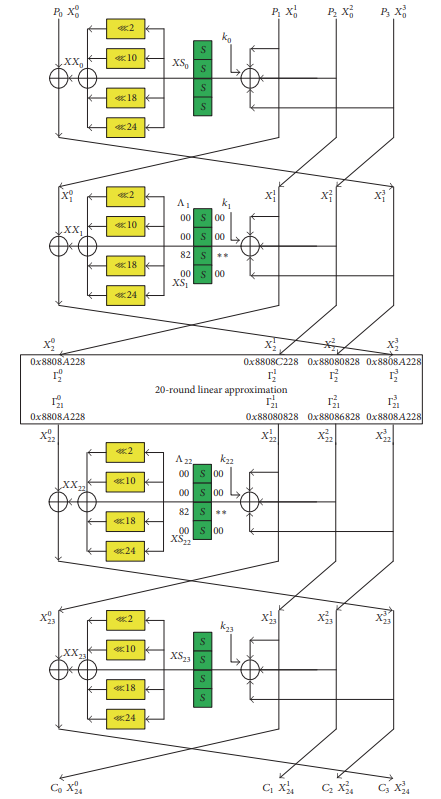
\includegraphics{diagramy/KeyRecoveryAttack.png}
  \caption{Atak odzyskiwania klucza na 24-rundowy SM4}
  \label{fig:KeyRecoveryAttack}
\end{figure}
